\section{Dise\~{n}o Orientado a Objetos}

A continuaci\'on se presenta el diseño orientado a objetos de todo el sistema implementado.

Dado que se quiere hacer hincapie en diferentes funcionalidades, se presentar\'a primero el sistema en su totalidad y luego se ir\'a explicando cada una de las partes m\'as importantes.


\bigskip
\begin{center}
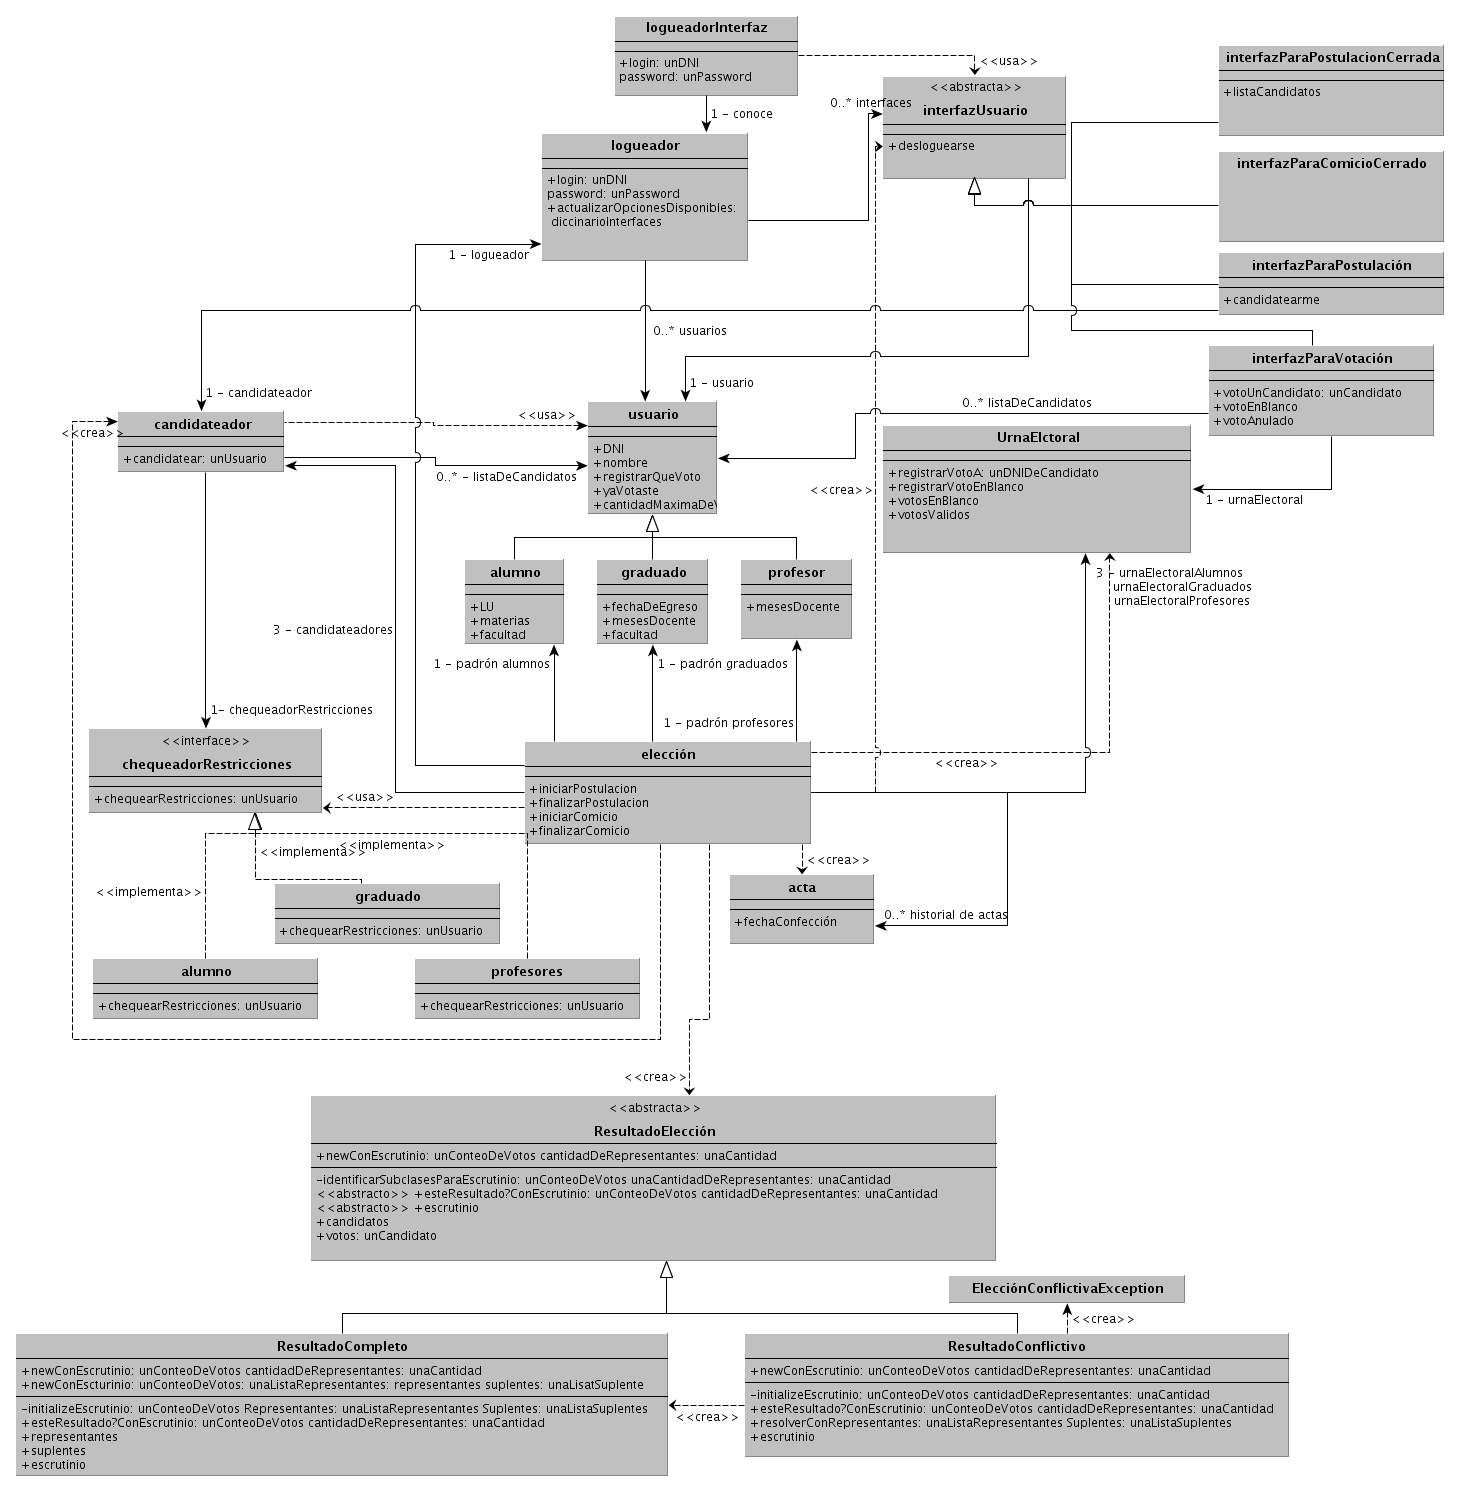
\includegraphics[scale=0.35]{diagramas/modeloClases.png} 
\end{center}
\bigskip


Antes de pasar a la explicaci\'on de cada una de las funcionalidades, se fundamentaran algunas decisiones de dise\~{n}o a un nivel m\'as alto y no dentro de una funcionalidad en particular.


\begin{itemize}
\item Desacomplamiento de las funcionalidades: El sistema VOX es lo suficientemente chico como para poder implementarlo sin la necesidad de un buen diseño y a\'un as\'i podr\'ia funcionar. Se podr\'ia hacer que existan pocos objetos que tengan muchas responsabilidades distintas sobre el sistema. Por ejemplo, podr\'ia haber un solo objeto que reifique a las elecciones en s\'i y que se encargue de la votaci\'on, de la postulaci\'on de candidatos y de todas las responsabilidades a implementar. Sin embargo, se decidi\'o realizar un dise\~{n}o orientado a objetos que se fundamente sobre las reglas vistas en la materia para obtener una mejor implementaci\'on del sistema. Es por esto que se decidi\'o no tener un objeto muy poco cohesivo, como ser\'ia esta elecci\'on multitarea, sino que se dividieron las responsabilidades en diferentes objetos que representen diferentes entes de la realidad. No es lo mismo querer postularse a candidato que querer emitir un voto, por lo que nos pareci\'o interesante tener estas funcionalidades bien desambiguadas. Adem\'as, esta decisi\'on tambien gana en otro tema muy importante para un buen diseño que es el bajo acomplamiento. Al separar las funcionalidades, el sistema es mucho m\'as tolerante a lo que puede suceder si solo una de estas funcionalidades cambia su comportamiento. En una elecci\'on pr\'oxima, la postulaci\'on a candidatos podr\'ia ser completamente diferente y esto no afectar a todo lo referente a la emisi\'on de un voto, o al sistema de logging.

\item Usuarios reificados. Charlando con los diferentes docentes de la materia, nos resulto interesante reificar el concepto de usuario del sistema. A priori un usuario pod\'ia ser simplemente un identificador, pero nos parecio adecuado reificar este concepto para tener informaci\'on que de otra forma corresponder\'ia a un sistema externo. Reificando el usuario y teniendo, por ejemplo en el caso del Alumno, la cantidad de materias, lo que podemos hacer es tener una sola interacci\'on con un sistema externo al comienzo de un acto electoral y de esa forma ya tener la informaci\'on necesaria en los objetos pertinentes, sin hacer m\'as complejo el dise\~{n}o. De hecho, nos parece que tambi\'en es una buena forma de mostrar la principal caracter\'istica de SCRUM, que es ser una metodolog\'ia iterativa-incremental; al modelarlo de esta forma, se trivializa un poco la interacci\'on con los sistemas externos, dejando esta funcionalidad para un sprint posterior. Por el momento, el modelo soporta el hecho de que al comenzar un acto electoral se cargan los padrones de los usuarios y con esto se obtiene la informaci\'on deseada. Esta forma de ingresar la informaci\'on de los usuarios es la funcionalidad que se podr\'ia incrementar en una iteraci\'on posterior.



\item Utilizaci\'on de interfaces. En variadas ocasiones se nos presento el problema de como modelar la interacci\'on entre todos los objetos del sistema y el usuario final que se encuentra detr\'as de la pantalla. Existen muchos mensajes que van a ser \emph{lanzados} seg\'un las acciones de un usuario del software en el mundo real. De esta forma, parecer\'ia que la interfaz gr\'afica tiene muchas responsabilidades porque necesita \emph{hablar} con muchos objetos. Por ejemplo para poder votar, parecer\'ia que el usuario del software tiene que hablar directamente con una urna, cuando no queremos eso ya que no es deseado que se pueda interactuar con el modelo interno del sistema. Por otro lado, tampoco es deseado que la interfaz gr\'afica de un software, como podr\'ia ser la pagina web de este sistema, tenga m\'as l\'ogica que simplemente renderizar lo que se le pide.

Es por esto que se decidio implementar una serie de interfaces para poder interactuar con el sistema de forma controlada. De esta manera, lo que sucede es que cuando un usuario del mundo real se loguea al sistema, la interfaz gr\'afica queda \emph{pegada} a una interfaz de uso del sistema, que ser\'a diferente dependiendo en la etapa que se encuentre la elecci\'on. Por ejemplo, si un usuario se loguea cuando la votaci\'on no esta abierta, sino que se estan postulando los candidatos, la interfaz gr\'afica solo tendr\'a comunicaci\'on con la interfazParaPostulaci\'on, la cual solo permitir\'a realizar acciones de postulaci\'on.

Tambi\'en se utiliz\'o una interfaz para el logging que ser\'a explicada cuando se explaye esta funcionalidad en particular.

\item Subclasificaci\'on de las interfaces.

Luego de resolver la necesidad de utilizar interfaces para poder interactuar entre el mundo real y el sistema externo, se vi\'o que se necesitaban diferentes interfaces seg\'un la \'epoca del acto electoral que transcurra, de modo que el sistema tenga un bajo acomplamiento y no haya un solo objeto manejando todo. Dado que se tienen diferentes interfaces, pero que todas representan la misma idea de ser la \emph{cara} del sistema frente al usuario real, nos pareci\'o pertinente realizar una subclasificaci\'on de las interfaces ya que esta idea se condice con el mundo real, en donde esta desambiguada la responsabilidad de efectuar la votaci\'on, la de postularse a candidato y las dem\'as.


\end{itemize}


\subsection{Logging}

En esta secci\'on se presenta todo lo referente al loggin al sistema. Al comenzar el diseño del tp, esta cuesti\'on no fue tomada como esencial ya que no era una de las funcionalidades b\'asicas a tener en cuenta en este sprint. Sin embargo, a medida que se fue desarrollando el diseño de todo el sistema, fue emergiendo la necesidad de explicar el modulo de logging, ya que resuelve cuestiones importantes para las dem\'as funcionalidades del sistema.

A continuaci\'on se presenta la parte del diagrama de clases que se refiere al logging para poder explicar de forma m\'as detallada las responsabilidades de cada clase y las reglas de diseño que nos llevaron a realizar el mismo.

\begin{center}
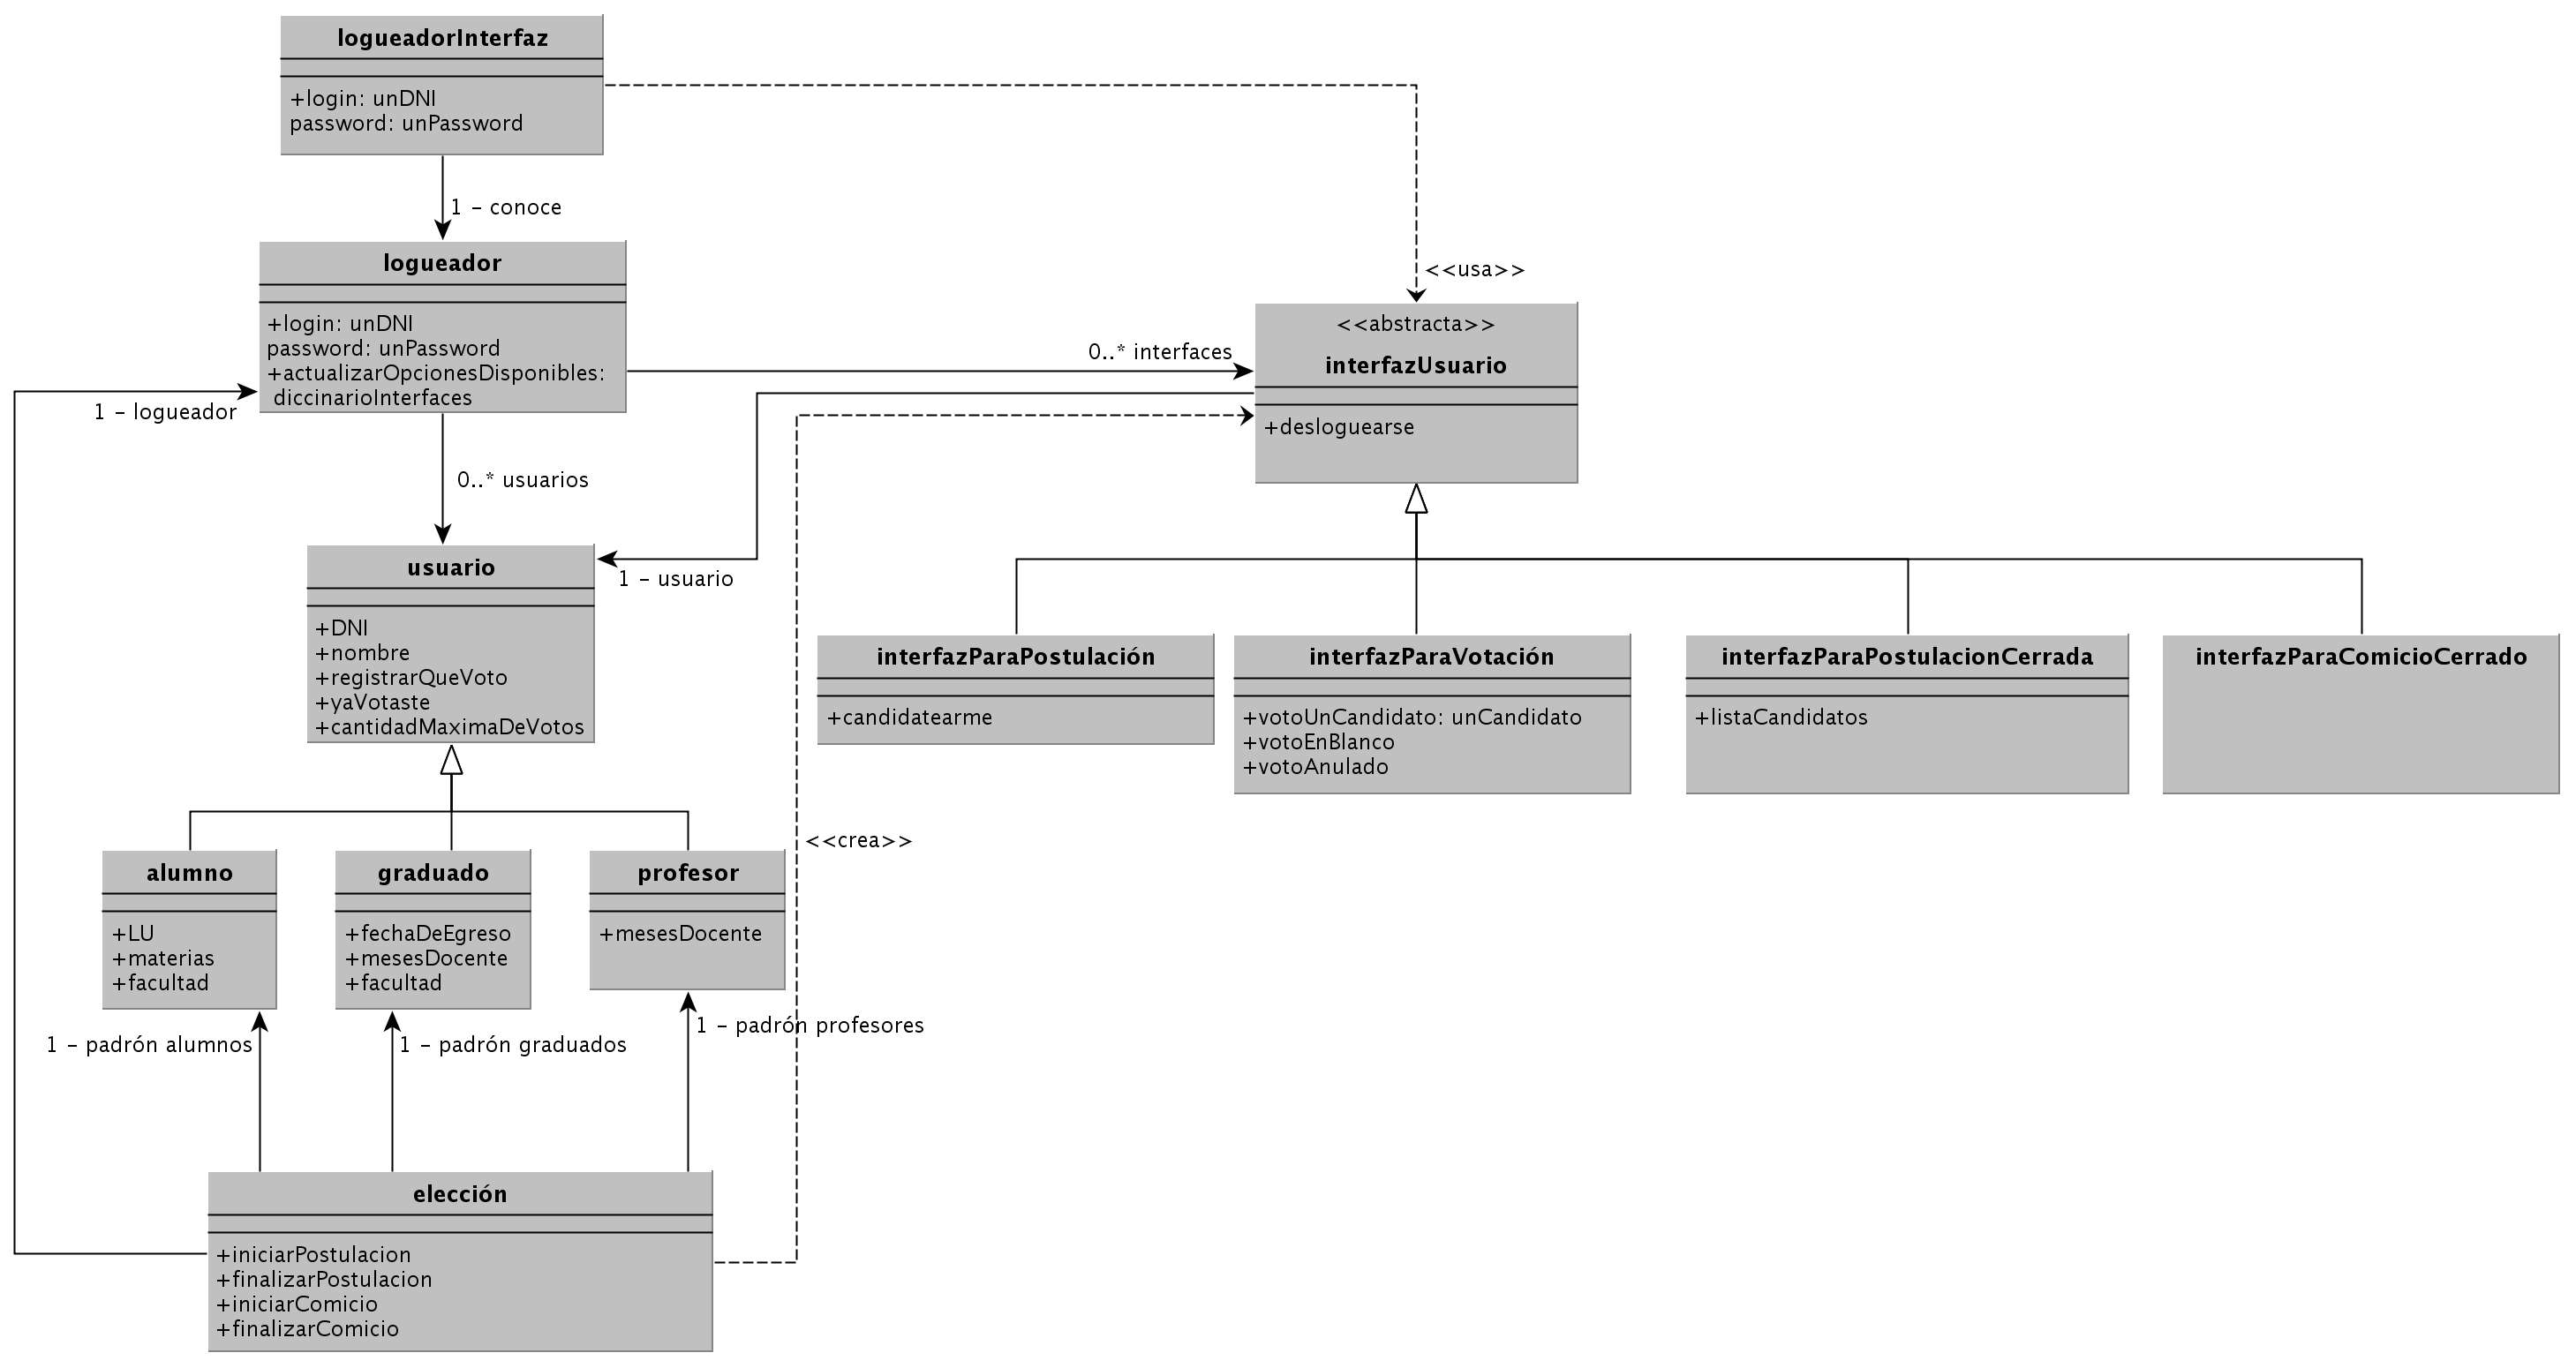
\includegraphics[scale=0.15]{diagramas/modeloDeClasesLogging.png}
\end{center}



\subsubsection{interfazLogueador}

La interfaz del logueador es un objeto que representa cual va a ser la interacci\'on del usuario real cuando quiera loguearse al sistema. Como se ver\'a en la explicaci\'on del logueador, este tiene ciertas funcionalidades e informaci\'on que no queremos que sea accesible ni manejable desde el exterior. Es por esto que se decidi\'o utilizar una interfaz de logueador con la siguiente responsabilidad.

\begin{itemize}
\item login: password:. Este mensaje contiene la \'unica responsabilidad de la interfaz de logueador, que es permitirle al usuario real loguearse en el sistema.
\end{itemize}

La principal idea de esta interfaz se basa en las reglas de diseño vistas durante las pr\'acticas de la materia que nos indica que es una buena decisi\'on poner una interfaz para poder interactuar con cosas interiores al modelo de una forma controlada. De esta forma un usuario real solamente podr\'a acceder a la funcionalidad de logging y no podr\'a acceder a otra informaci\'on interesante que pueda tener el modelo interno de datos. 

\subsubsection{Logueador}

El logueador es un objeto que tendra como responsabilidad manejar todo lo pertinente al ingreso al sistema de una persona. Si bien su responsabilidad principal es el mensaje de logging, maneja otras informaciones necesarias para el loggin como saber en que etapa de las elecciones estamos. Estas son cosas que no queremos que el usuario real pueda acceder, por lo cual justifica la necesidad de una interfaz para interactuar con este objeto.

El logueador funciona de la siguiente manera. El objeto sabe que interfaz le corresponde a cada usuario, por lo que el mismo tiene una representaci\'on interna de las asociaciones entre los usuarios del sistema y las interfaz de usuario. Esta representaci\'on se va modificando dependiendo el estado de las elecciones actuales (postulaci\'on, idle, votaci\'on, etc).
Lo que hace el logueador es entonces, cuando loguea a un usuario, devolver una interfaz de usuario seg\'un la representaci\'on que tenga de la asociaci\'on entre el usuario que quiere loguear y la interfaz que le corresponde. Es decir, si la elecci\'on est\'a en \'epoca de votaci\'on entonces los usuarios del sistema estaran asociados a interfaces de usuario que en realidad son interfaces para votaci\'on. De esta forma, lo que hace el logueador es simplemente devolver la interfaz que esta asociada para que se puede interactuar con el sistema, por ejemplo para votar, mediante esta interfaz que es nuestra fachada para interactuar con el sistema interno.

El logueador resuelve esta situaci\'on mediante los siguientes mensajes:

\begin{itemize}
\item login: password:. Es el mensaje esencial de un logueador que es justamente su funci\'on principal, la de loguear. Este mensaje va a ser utilizado desde la interfaz de logueador que es la \'unica manera que tiene un usuario real para hablar.
\item actualizarOpcionesDisponibles:. Este mensaje es el que permite asociar a los usuarios con las diferentes interfaces disponibles para interactuar con el sistema. De esta manera, los usuarios siempre tendr\'an una interfaz de usuario asociada, pero al utilizar este mensaje, esas interfaces podr\'an cambiar, asociandose con la interfaz necesar\'ia para la \'epoca de la elecci\'on pertinente. Entonces, a partir del uso de este mensaje, cuando los usuarios se logueen, podran interactuar con VOX mediante la interfaz que les corresponda con ese per\'iodo de las elecciones. Entonces si utilizamos este mensaje para asociar a los usuarios con una interfaz de postulaci\'on, lo que estaremos logrando es que el usuario cuando se loguee solo puede interactuar con el sistema mediante una interfaz de postulaci\'on que solo tendr\'a como opci\'on de funcionalidad posible el hecho de candidatearse; ya que por la \'epoca de las elecciones en las que se encuentra el sistema, no se deber\'ia poner hacer otra cosa.
\end{itemize}

\subsubsection{elecci\'on}

En esta funcionalidad en particular, la de loguearse, las responsabilidades de esta clase se basan en manejar los tiempos de las elecciones para saber que se puede hacer con el sistema en este momento. La clase elecci\'on es el principal punto de interacci\'on para un administrador del sistema. Lo cual probablemente inducir\'ia a tener una interfaz para administrador que ser\'a adherida al modelo, en caso de necesitarla, en otra iteraci\'on del presente desarrollo.

Luego, este objeto es responsable de indicar en que etapa de las elecciones esta el sistema, mediante la asignaci\'on de las diferentes interfaces a los usuarios. Los mensajes para cumplir con estas responsabilidades son:

\begin{itemize}
\item iniciarPostulacion:. Este mensaje se encarga de hablar con el logueador para que ahora todos los usuarios tengan asociada una interfaz para postulaci\'on.
\item cerrarPostulacion:. Este mensaje sirve para que cuando falten 14 dias para la elecci\'on la postulaci\'on se cierre y ahora los usuarios reales no puedan interactuar con la interfaz para postulaci\'on, sino que solo pueden ver los candidatos.
\item iniciarComicio: Este mensaje sirve para asociar a los usuarios con las interfaces de votaci\'on de manera que sea posible interactuar con el sistema para poder emitir un voto.
\item FinalizarComicio: Con este mensaje se da por cerrada una elecci\'on y esto influye en el sistema de loggin por que ahora los usuarios reales solo podr\'an interactuar con una interfaz que lo \'unico que les deja hacer es ver los resultados de la elecci\'on. 
\end{itemize}




\bigskip

A continuaci\'on, se presenta un diagrama de secuencia que sirve para entender de forma din\'amica la interacci\'on entre los diferentes objetos en una traza particular para la funcionalidad de logueo.

\begin{center}
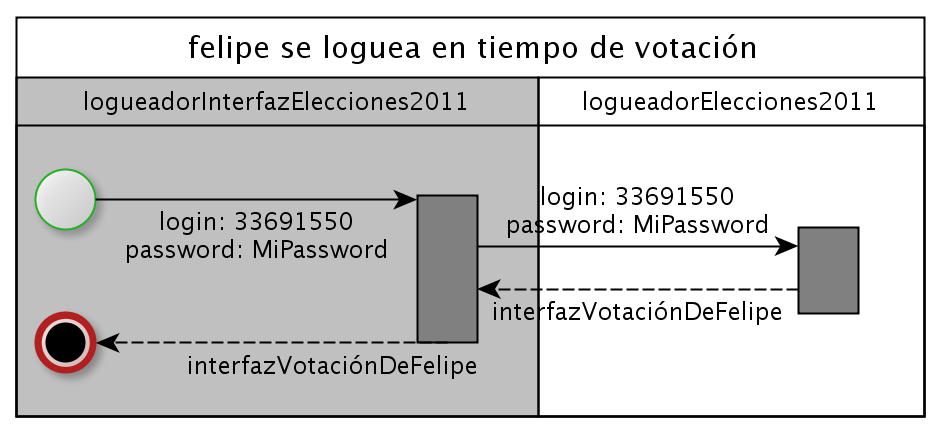
\includegraphics[scale=0.3]{diagramas/diagramaSecuenciaSeLogueaUnAlumno.png}
\end{center}





Por \'ultimo, se presenta un diagrama de objetos, para poder identificar las colaboraciones entres los diferentes objetos del sistema en un momento en particular.

\begin{center}
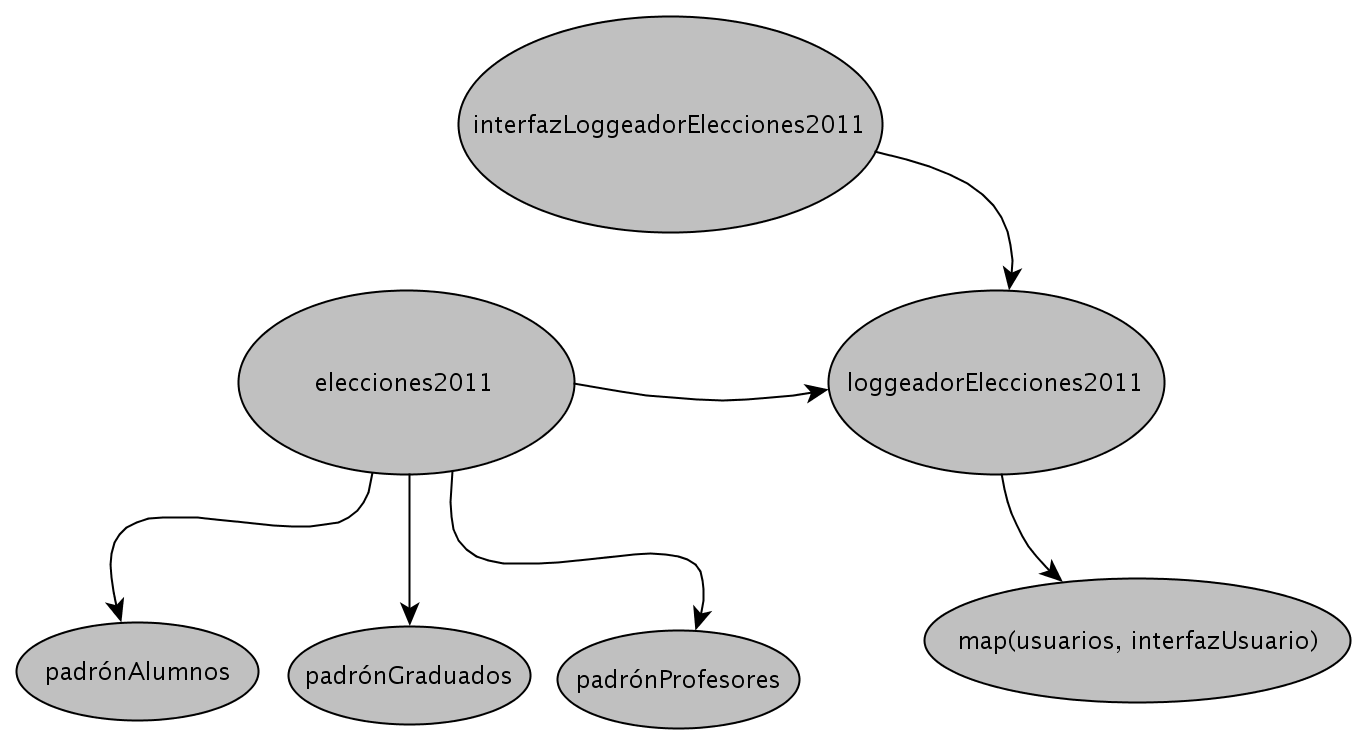
\includegraphics[scale=0.3]{diagramas/modeloDeObjetosLogging.png}
\end{center}





\subsection{Postulaci\'on a candidato}

En esta secci\'on se presenta la funcionalidad particular de postularse para ser candidato en las elecciones.


Para esto, se reproduce el subconjunto de clases del diagrama original, que corresponden a esta secci\'on en particular.




\subsubsection{candidateador}

La idea del candidateador es tener un objeto que reifique el concepto que se tendr\'ia en una votaci\'on sin un sistema inform\'atico, en el cual un potencial candidato ir\'ia hacia una persona dedicada a la tarea de la postulaci\'on para postularse. Esta persona ser\'ia la encargada de, por un lado, mirar que el aspirante no aparezca ya en la lista de candidatos, de forma que no pueda haber un candidato postulado dos veces. Luego, esta persona ser\'ia tambi\'en la encargada de utilizar alg\'un sistema externo, o alg\'un catalogo de legajos, para fijarse si el potencial candidato cumple los requisitos necesarios. Nos parece que la tarea de chequear las restricciones es una responsabilidad grande como para asignarsela a un objeto dedicado solamente a eso. Es por esto que en este punto, el candidateador solo chequear\'a las restricciones colaborando con otro objeto que se encargar\'a del chequeo propiamente dicho.

Luego, para resolver las responsabilidades de una forma bien cohesiva, se tiene un \'unico mensaje:

\begin{itemize}
\item candidatear:. Este mensaje es la \'unica responsabilidad que tiene el objeto, recibe un usuario a candidatear y se fija si ya pertenece a su lista interna. Adem\'as, en la implementaci\'on de este mensaje, el objeto candidateador colabora con el Chequeador para que este le diga si el postulante cumple con los requisitos. Dependiendo el caso del postulante, el candidateador lo sumar\'a a la lista de candidatos o no.
\end{itemize}


\subsubsection{interfazParaPostulaci\'on}

Esta interfaz tiene un comportamiento similiar a todas las dem\'as interfaces de usuario. Lo que hace es dar una puerta de entrada al sistema para poder interactuar con el subsistema de postulaci\'on, pero sin tener acceso a mensajes o informaciones internas que no queremos que un usuario real pueda acceder. Si el usuario real pudiese interactuar directamente con el candidateador, podr\'ia eventualmente tener acceso a la lista de candidatos, situaci\'on que no queremos que ocurra. Es por esto que la \'unica responsabilidad de la interfaz es tener un mensaje para candidatear a un usuario, y se encarga de enviar esta petici\'on al candidateador real.


\subsubsection{Chequeador de Restricciones}

El problema de saber si un postulante cumple con los requisitos para ser candidato no es una responsabilidad menor, sobretodo por el hecho de que queremos darle extensibilidad a esta parte del diseño, permitiendo que cambien los reglamentos por los cuales se chequean los requisitos.

Es por esto que existe el objeto chequeador de restricciones para desacoplar esta responsabilidad del candidateador. La clase chequeadorDeRestricciones adem\'as se encuentra subclasificada en chequeador de alumnos, chequeador de graduados y chequeador de profesores. De esta manera, los diferentes candidateadores conoceran diferentes chequeadores de forma de poder delegar las responsabilidad del chequeo en estos.

Cada tipo de chequeador diferente, chequea mediante el reglamento propio a cada claustro, de forma que se puede desacoplar el chequeo de un graduado del de un alumno o un profesor.





\bigskip

A continuaci\'on se presenta la traza correspondiente a un graduado que se quiere candidatear mediante un diagrama de secuencia. De esta forma, se pueden ver las interacciones que tienen los diferentes objetos cuando un graduado se quiere candidatear.

\begin{center}
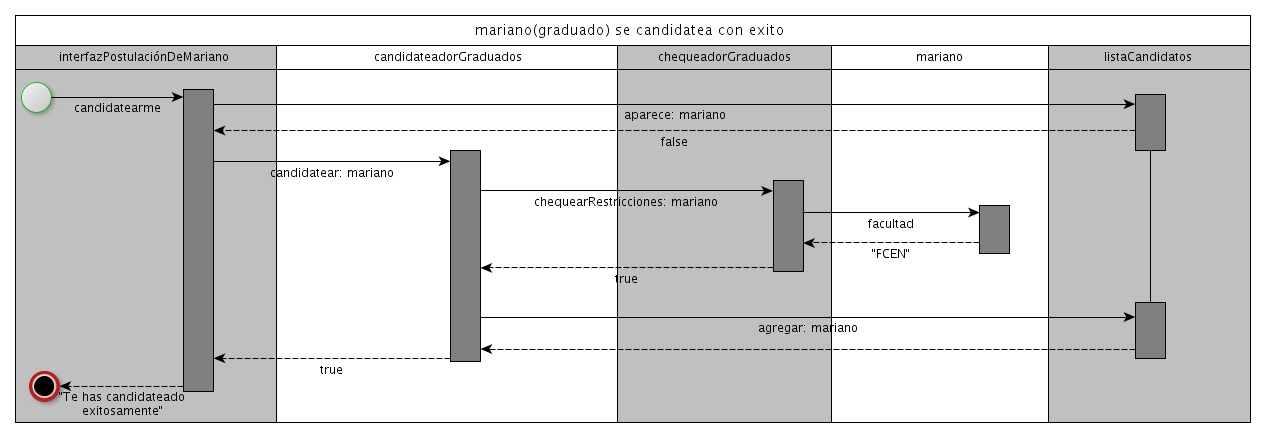
\includegraphics[scale=0.35]{diagramas/diagramaGraduadoSeCandidateaExitosamente.png}
\end{center}



\bigskip

Por \'ultimo, se presenta un diagrama de objetos para esta funcionalidad.

\begin{center}
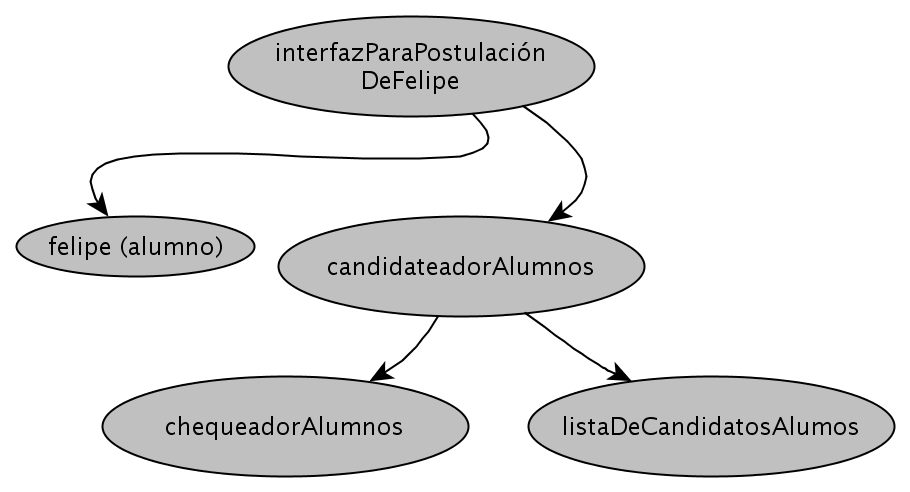
\includegraphics[scale=0.3]{diagramas/modeloDeObjetosCandidatearse.png}
\end{center}

\subsection{Votaci\'on}

%clase

En esta secci\'on se presenta un subconjunto de las clases del diagrama original que son pertinentes al problema de la votaci\'on.

A continuaci\'on se reproduce dicho subconjunto separado del diagrama original, para luego poder explicitar cada decisi\'on tomada sobre cada una de las clases presentes.

\begin{center}
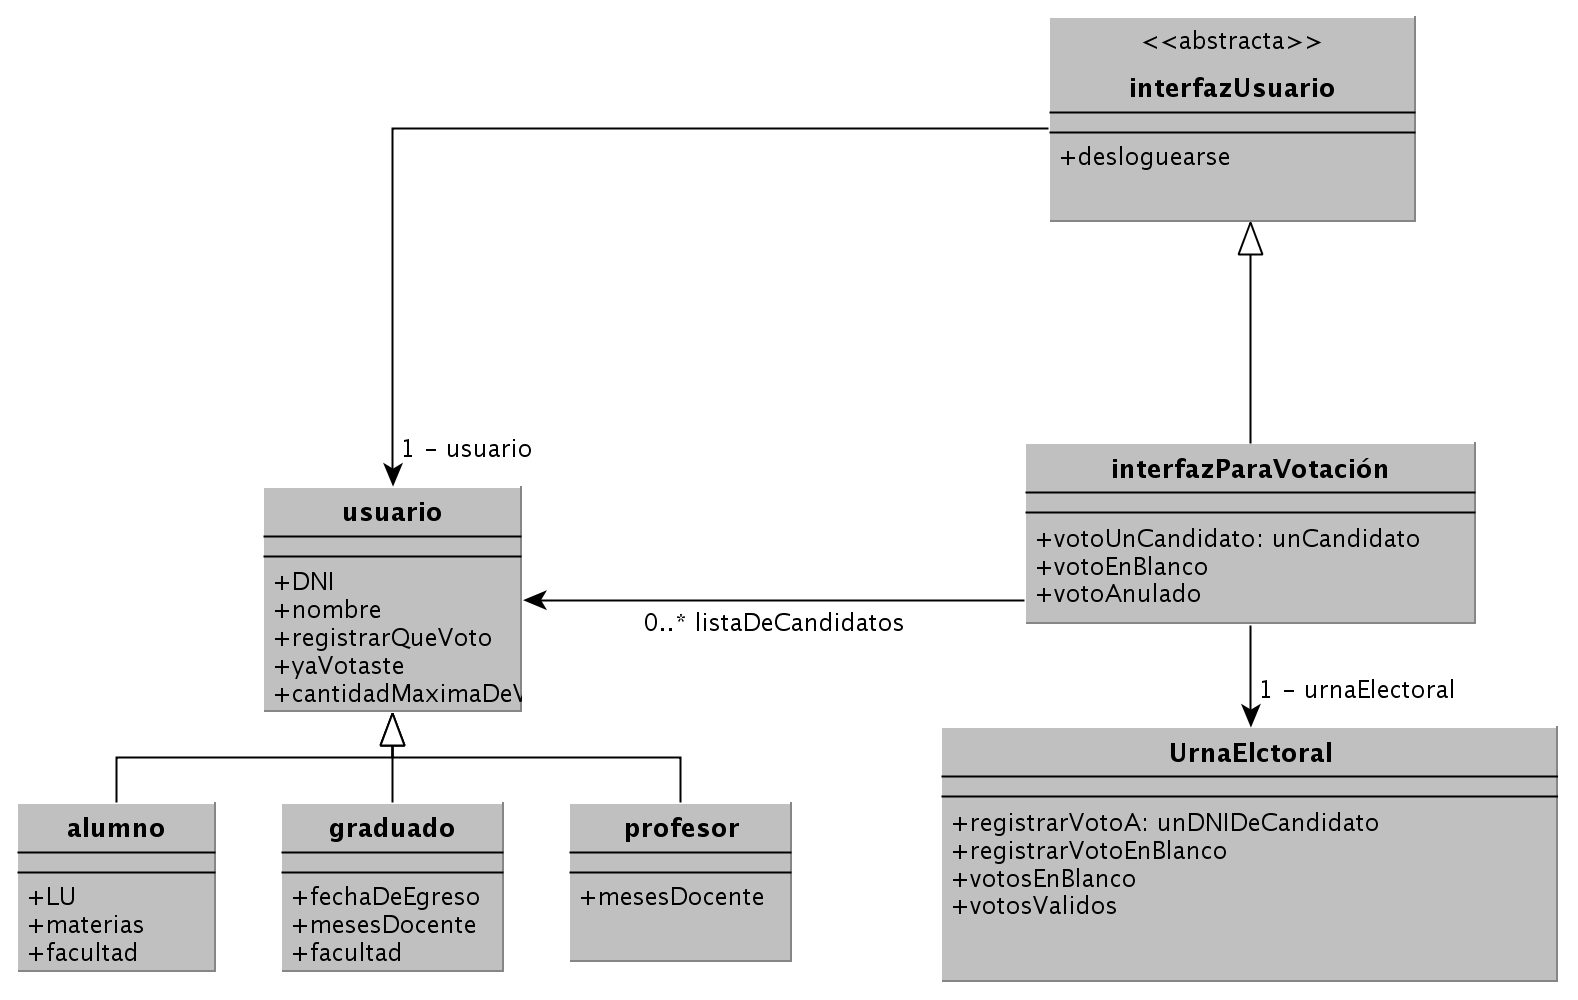
\includegraphics[scale=0.3]{diagramas/modeloDeClasesVotacion.png}
\end{center}

\subsubsection{Usuario}

El usuario representa a un posible votante o candidato, pero en este caso, solo nos importa el mismo como votante. La entidad del mundo real a la que hace referencia es el votante al momento de iniciarse el proceso electoral. Cualquier usuario debe ser capaz de responder a los mensajes DNI, nombre, registrarQueVoto, yaVotaste. Los mismos se utilizan para:

\begin{itemize}
\item DNI: Es un mensaje esencial al usuario, que lo identica como objeto entre los de su misma clase. El mismo hace referencia directa a un usuario del sistema, por lo que tambi\'en servir\'a para hacer el recuento de votos. Es decir que los votos en el sistema se dividir\'an de acuerdo al DNI del candidato al que hacen referencia.
\item nombre: Responde al nombre de la persona real que hace referencia el usuario.
\item registrarQueVoto: Es un mensaje que permite registrarle al usuario que ya vot\'o para que no pueda volver a votar.
\item yaVotaste: Es un mensaje que permite preguntarle al usuario si ya vot\'o. Sirve para cumplir con la restricci\'on de que un usuario no pueda volver a sufragar.
\item cantidadMaximaDeVotos: Es un mensaje que responde cuantos postulantes puede votar un usuario.
\end{itemize}

En cuanto a los mensajes presentandos anteriormente, desde un punto de vista estrictamente paradigm\'atico, no queda claro que sea responsabilidad del usuario saber que ya vot\'o. Sin embargo, se decidi\'o hacerlo de esta forma para reducirle la complejidad al modelo.

Por el mismo motivo se encuentra el mensaje cantidadMaximaDeVotos que, bajo el consejo de Fernando Astesuain, se puso dentro del usuario para que sea simple la votaci\'on. Directamente se puede votar una collection de candidatos y chequar cuantos puede votar realmente mediante este mensaje.

En el diagrama, se puede observar que los usuarios estan subclasificados en Alumno, Graduado y Profesor. Esta subclasificaci\'on no es muy relevante a esta parte del problema, ya que concierne a las restricciones para las postulaciones de candidato. Como se ver\'a luego, la interfaz de votaci\'on es la que sabe si se trata de un alumno o graduado, o si se trata de un profesor, para saber si puede votar una o dos veces.

Esto lo hicimos de esta forma para seguir una de las principales reglas de diseño en cuanto a que los objetos sean cohesivos. Buscamos tener un usuario que no sepa hacer cosas como votar, o candidatearse o tener otras responsabilidades; sino que pueda responder mensajes muy b\'asicos con pocas responsabilidades.

\subsubsection{urnaElectoral}

La urnaElectoral reifica el concepto de urna que se tendr\'ia en el dominio del problema. La urna es la encargada de llevar los votos de cada una de las votaciones que haya. Una primer idea hab\'ia sido subclasificar la urna dependiendo del claustro a la que pertenezca. Sin embargo, con la busqueda de tener objetos bien cohesivos, nos dimos cuenta que realmente no importa a que claustro pertenezca la urna, sino que simplemente debe guardar los votos de la elecci\'on para la que fue asignada. Esto quiere decir que el sistema problablemente tenga m\'as de una urna, que van a ser una para Alumnos, una para Graduados y una para Profesores; pero estas urnas van a hacer equivalentes, son todas instancias de la misma clase porque las responsabilidades que tienen son las de ser una urna independientes del claustro. Dicho esto, las responsabilidades de una urna son:

\begin{itemize} 
\item registrarVotoA:, Este mensaje lo que hace es justamente \emph{meter} un voto en la urna. Dado que lo \'unico que queremos es registrar el voto, la urna solo necesita saber a quien se esta votando.
\item registrarVotoEnBlanco. Este mensaje deja registrar un voto en blanco. Nos parece que es una buena decisi\'on de diseño desambiguar el voto en blanco respecto del voto v\'alido, para tener conceptos diferentes reificados de forma diferente y que un voto en blanco no sea simplemente un voto a nil de un voto v\'alido.
\item votosEnBlanco. Es el mensaje que representar\'ia abrir la urna y poder contar los votos en blanco que hubo.
\item votosValidos. Es un mensaje que nos devuelve una lista de candidatos junto con la cantidad de votos que tuvieron durante la elecci\'on.
\end{itemize}


\subsubsection{interfazParaVotaci\'on}

La interfaz para votaci\'on es el objeto que principalmente maneja el sufragio de un usuario. Representa lo que en el mundo real ser\'ia la autoridad de mesa cuando el votante va a emitir su voto. Desde este punto de vista, la responsabilidad de los objetos de esta clase es manejar el momento del voto en s\'i. Este objeto intenta ser lo m\'as cohesivo posible responsabilizandose solamente por el acto de la votaci\'on, mientras que las dem\'as funcionalidades quedan como responsabilidad de otros objetos. Para lograr encargarse de estas cosas, las instancias de esta clase saben responder los siguientes mensajes:

\begin{itemize}
\item votarCandidatos:. Este mensaje toma una colecci\'on de candidatos a votar y trata de emitir el voto. Al tratar de emitir el voto, se chequea que el usuario no haya votado, y se chequea que la cantidad de gente que esta queriendo votar sea menor o igual a la m\'axima cantidad de personas que puede votar. Si se puede emitir el voto, entonces esta interfaz es la responsable de comunicarse con la urna para \emph{introducirle} un voto por cada candidato votado, as\'i como tambi\'en se responsabiliza de indicar que el usuario ya vot\'o.
\item votoEnBlanco. Este mensaje se encuentra para que un usuario tenga la posibilidad de votar en blanco. Nuevamente argumentamos que desde un punto de vista del paradigma de objetos, nos parece bien desambiguar los votos en blanco para que no haya colisi\'on de conceptos del dominio del problema, como nos indica una de las mencionadas reglas de dise\~{n}o.
\end{itemize}




\bigskip

Si bien el diagrama de clases, m\'as la explicaci\'on del mismo, nos da una idea aproximada de como interact\'uan los objetos entre s\'i, presentaremos a continuaci\'on un diagrama de secuencia que indica como ser\'ia una traza posible de las interacciones din\'amicas entre diferentes objetos involucrados en el proceso de votaci\'on.

\begin{center}
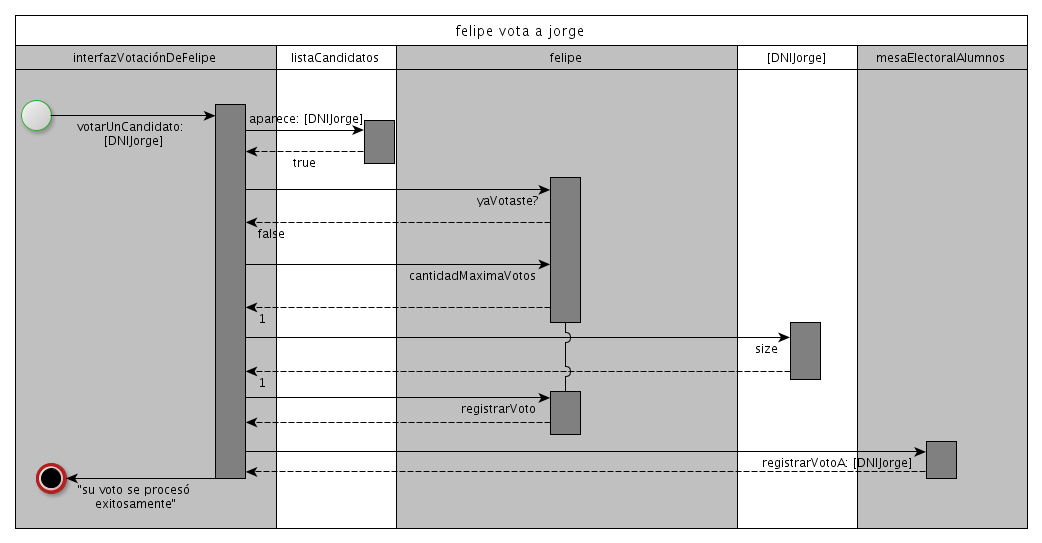
\includegraphics[scale=0.4]{diagramas/diagramaSecuenciaVotaUnAlumno.png}
\end{center}


\bigskip

Por \'ultimo, nos parece interesante mostrar un diagrama de instancias que resalte como ser\'ia la relaci\'on de conocimiento entre diferentes objetos en el transcurso de una votaci\'on.

En este caso se presenta una caso donde un Alumno, un Graduado y un Profesor quieren emitir su voto.

\begin{center}
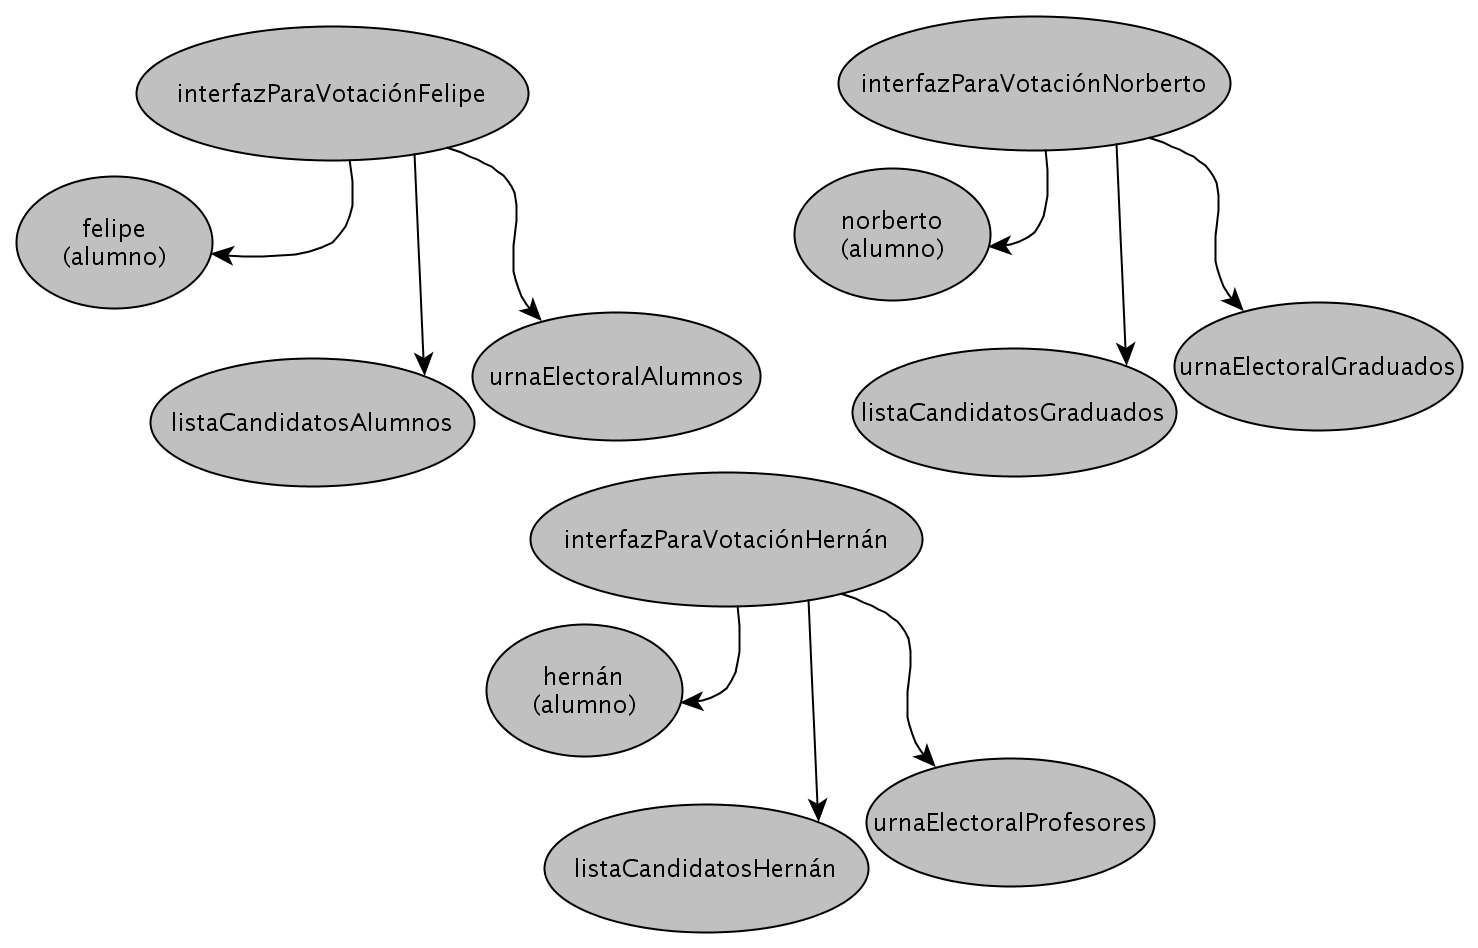
\includegraphics[scale=0.25]{diagramas/modeloDeObjetosVotacion.png}
\end{center}


\subsection{Clausura del acto electoral}

En esta secci\'on, se mostrar\'a como se atac\'o el diseño correspondiente al cierre del acto electoral, en el cual se tienen que resolver algunas situaciones como la generaci\'on de actas y la resoluci\'on de los conflictos.

A continuaci\'on se reproduce el sector del diagrama de clases correspondiente a la clausura del acto electoral.

\begin{center}
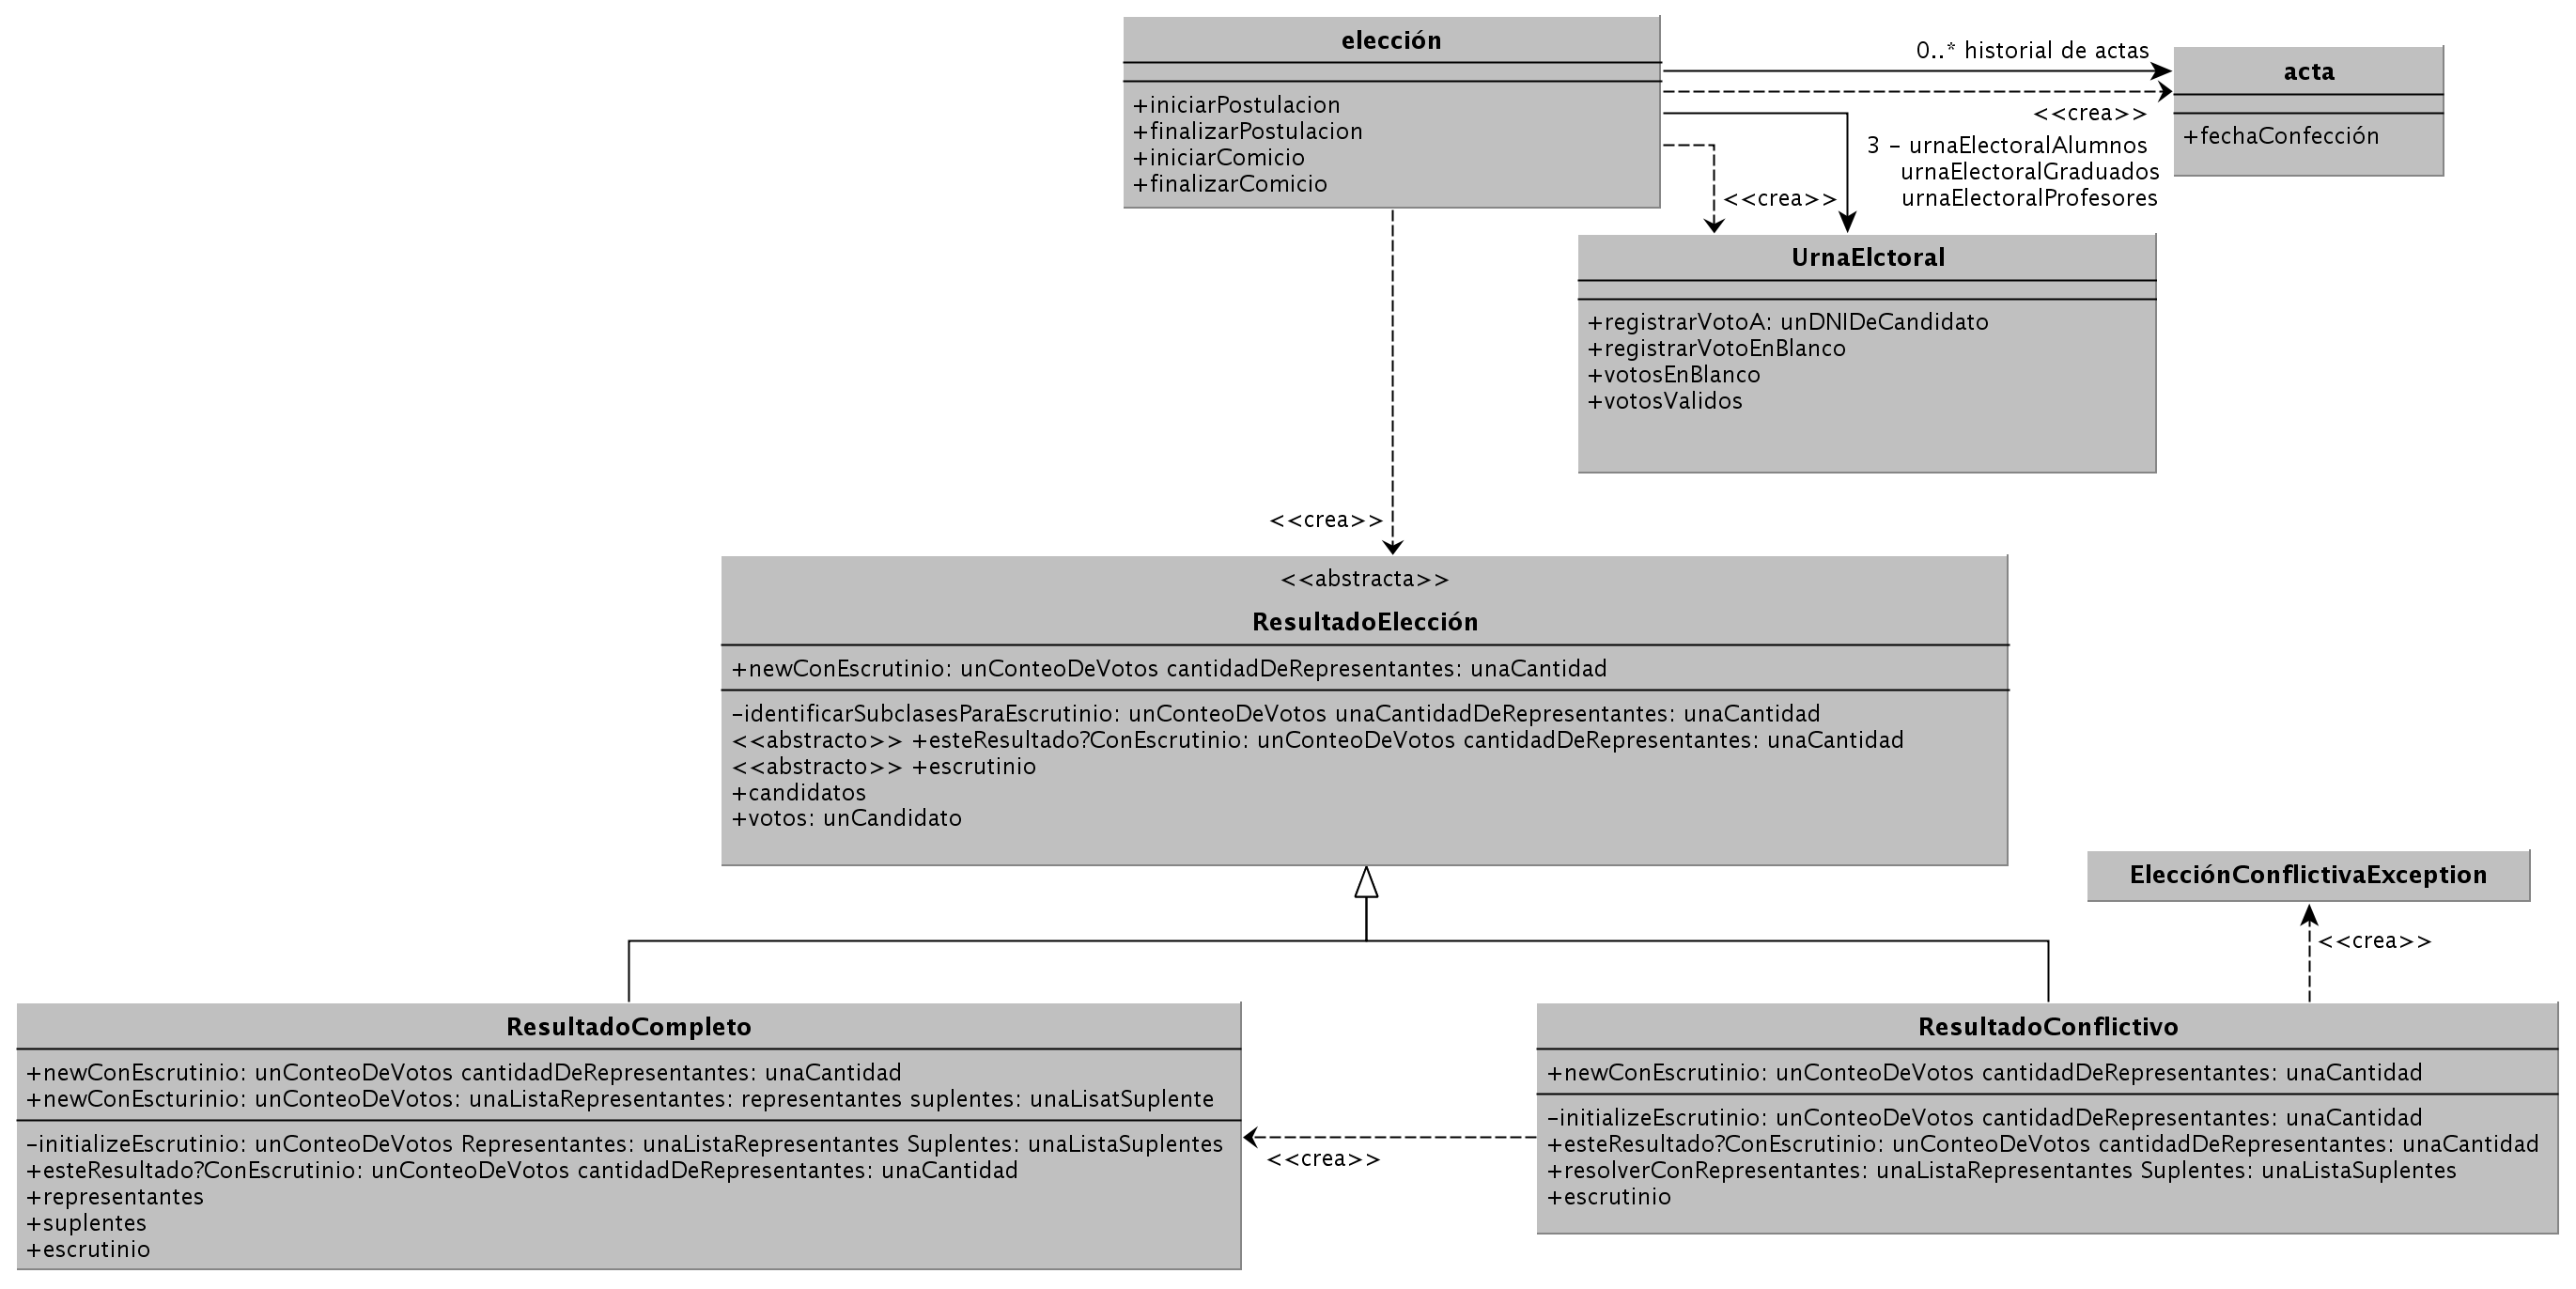
\includegraphics[scale=0.19]{diagramas/modeloDeClasesResultados.png}
\end{center}


Lo que se busca en esta simple jerarquía es reificar los distintos posibles resultados de una votación correspondiente a un claustro. Uno de los objetivos al diseñar este módulo fue permitir extender fácilmente la lógica de Vox agregándo resolución automática de conflictos a las funcionalidades provistas.

La implementación entregada como prueba de concepto permite agregar resolución a un tipo de conflicto en particular sin modificar en absoluto el código existente. Esto se puede realizar agregando una subclase de ResultadoEleccion que devuelva una instancia de True al mensaje esteResultado?conEscrutinio: cantidadDeRepresentantes: . La manera en la que lo implementamos fue utilizando una ligera modificación del patrón Factory Method, cuya implementación fue mostrada en las clases teóricas como ejemplo de un idiom de Smalltalk. 

Por mencionar un ejemplo, se podrían resolver automáticamente los conflictos de empate sin modificar el comportamiento en los casos de falta de candidatos, siendo conflictos de empate en los que ocurre un empate de votos entre dos candidatos y no es posible distinguir cuál de los dos debe ser representante y cuál suplente.

\subsubsection{ResultadoEleccion}


La clase ResultadoEleccion representa el resultado de una elección y como tal no existe una instancia concreta del mismo, es por eso que resulta una clase abstracta. 

\subsubsection{ResultadoCompleto}
La clase ResultadoCompleto por su parte representa el resultado de una elección en la que se pudo determinar sin ambigüedades cuáles serán los representantes y cuáles los suplentes, ya sea debido a que la misma no existió desde un principio o porque la misma fue resuelta ya sea por la junta electoral o eventualmente por algún algoritmo incorporado a Vox.


\subsubsection{ResultadoConflictivo}
Por último, la clase ResultadoConflictivo representa el resultado de una elección a partir del cual no puede automáticamente deducirse qué candidatos deberían ser representantes y cuáles suplentes. Esta última admite la resolución manual del conflicto ingresando una lista de representantes y de suplentes. No se aplican restricciones sobre la lista de representantes y suplentes, excepto que la longitud de la lista de representantes debe ser exactamente la correspondiente a la elección.




Se está suponiendo que el único eje de cambio en la resolución automática de conflictos es respecto del tipo de conflictos y no de los claustros. La razón para tal suposición es que se cree que tal resolución deberá ser lo más objetiva posible y por lo tanto recurrirá a métodos estocásticos en el caso de empate, por ejemplo, o incluirá automáticamente como representantes incluso a aquellos candidatos que no hayan obtenido el 10 porciento de votos usualmente requerido.

Pese a esta suposición, es importante mencionar que el diseño podría modificarse ligeramente para permitir la inclusión algoritmos de resolución automática de conflictos diferentes para cada claustro. Una buena razón para no hacerlo inicialmente y sacrificar dicha cualidad es que se prefiere priorizar la cohesión de la clase ResultadoEleccion y sus subclases, manteniendo un único eje de cambio.


\subsubsection{EleccionConflictivaException}
EleccionConflictivaException es una excepción que será lanzada si se manda el mensaje representantes o suplentes a una instancia de la clase ResultadoConflictivo. De esta manera se permite manejar este tipo de situaciones solicitando la intervención de un usuario administrador, que actuará en nombre de la junta electoral, indicando una resolución manual al conflicto surgido. Cualquier instancia de esta clase responde al mensaje parameter con la instancia de ResultadoConflictivo que lanzó la excepción.



Para la mejor comprensión de la implementación entregada es importante comentar que la semántica de ResultadoEleccion $>>$ newConEscrutinio: cantidadDeRepresentantes:  es crear una instancia de una de sus subclases cuando dicha subclase es la única que responde afirmativamente al mensaje esteResultado?conEscrutinio: cantidadDeRepresentantes:. De no existir una subclase que responda afirmativamente a dicho mensaje se retorna una instancia de ResultadoConflictivo. Por esta razón ResultadoConflictivo responde siempre negativamente a dicho mensaje. Si existieran varias subclases de ResultadoEleccion que fueran compatibles con los parámetros, se lanza otra excepción, que no es incluída en los diagramas de clases porque consideramos que no es esencial al modelo, sino accidental y debida a la implementación de la prueba de concepto.


\bigskip


El siguiente diagrama de secuencia muestra las colaboraciones al darse por finalizados los comicios. En este caso no surgieron ambigüedades en cuanto a los resultados. 


% Tras varias colaboraciones producto de la finalización de los comicios que no son incluídas, "mesaElectoral" envía el mensaje 
% "newConEscrutinio: conteoDeVotos cantidadDeRepresentantes: cantidad" a la clase ResultadoEleccion, la cual se envía a sí misma el mensaje "identificarSubclasesParaEscrutinio: conteoDeVotos cantidadDeRepresentantes: cantidad". 
% 
% Dicho envío de mensaje genera la ejecución de un nuevo método por parte del mismo objeto (en el grafiquito tiene que aparecer otra cajita, como cuando Nicolás mostró el patrón visitor), en el cual se envía a las subclases de ResultadoEleccion el mensaje "esteResultado?conEscrutinio: conteoDeVotos cantidadDeRepresentantes: cantidad", al cual ResultadoCompleto responde afirmativamente y ResultadoConflictivo responde negativamente.
% 
% Tras esto se termina la ejecución del segundo método de ResultadoEleccion, que retorna una lista que contiene únicamente a la clase ResultadoCompleto y devuelve de esta manera la ejecución al primer método invocado.
% 
% Posteriormente se llama al método ResultadoCompleto $>>$ newConEscrutinio: conteoDeVotos cantidadDeRepresentantes: cantidad
% que realizar varios cómputos, para generar las listas de representantes y suplentes, las cuales incluye como parámetros del mensaje "newConEscturinio: conteoDeVotos Representantes: representantes Suplentes: suplentes" que se envía a sí misma.
% 
% Esto genera la ejecución de un segundo método de ResultadoCompleto, en la cual se crea una instancia concreta, "resultadoEleccionEstudiantes2011", a la cuál se envía el mensaje "initializeEscrutinio: conteoDeVotos Representantes: representantes Suplentes: representantes". La respuesta a este mensaje es la "resultadoEleccionEstudiantes2011" en sí misma, así como también es la respuesta a todos los mensajes todavía siendo procesados.
% 
% 
% Posteriormente "mesaElectoralEstudiantes" envía a "resultadoEleccionEstudiantes2011" el mensaje representantes, al cuál responde con la lista que contiene a los usuarios correspondientes a Federico Pousa y Facundo Carrillo.


\begin{center}
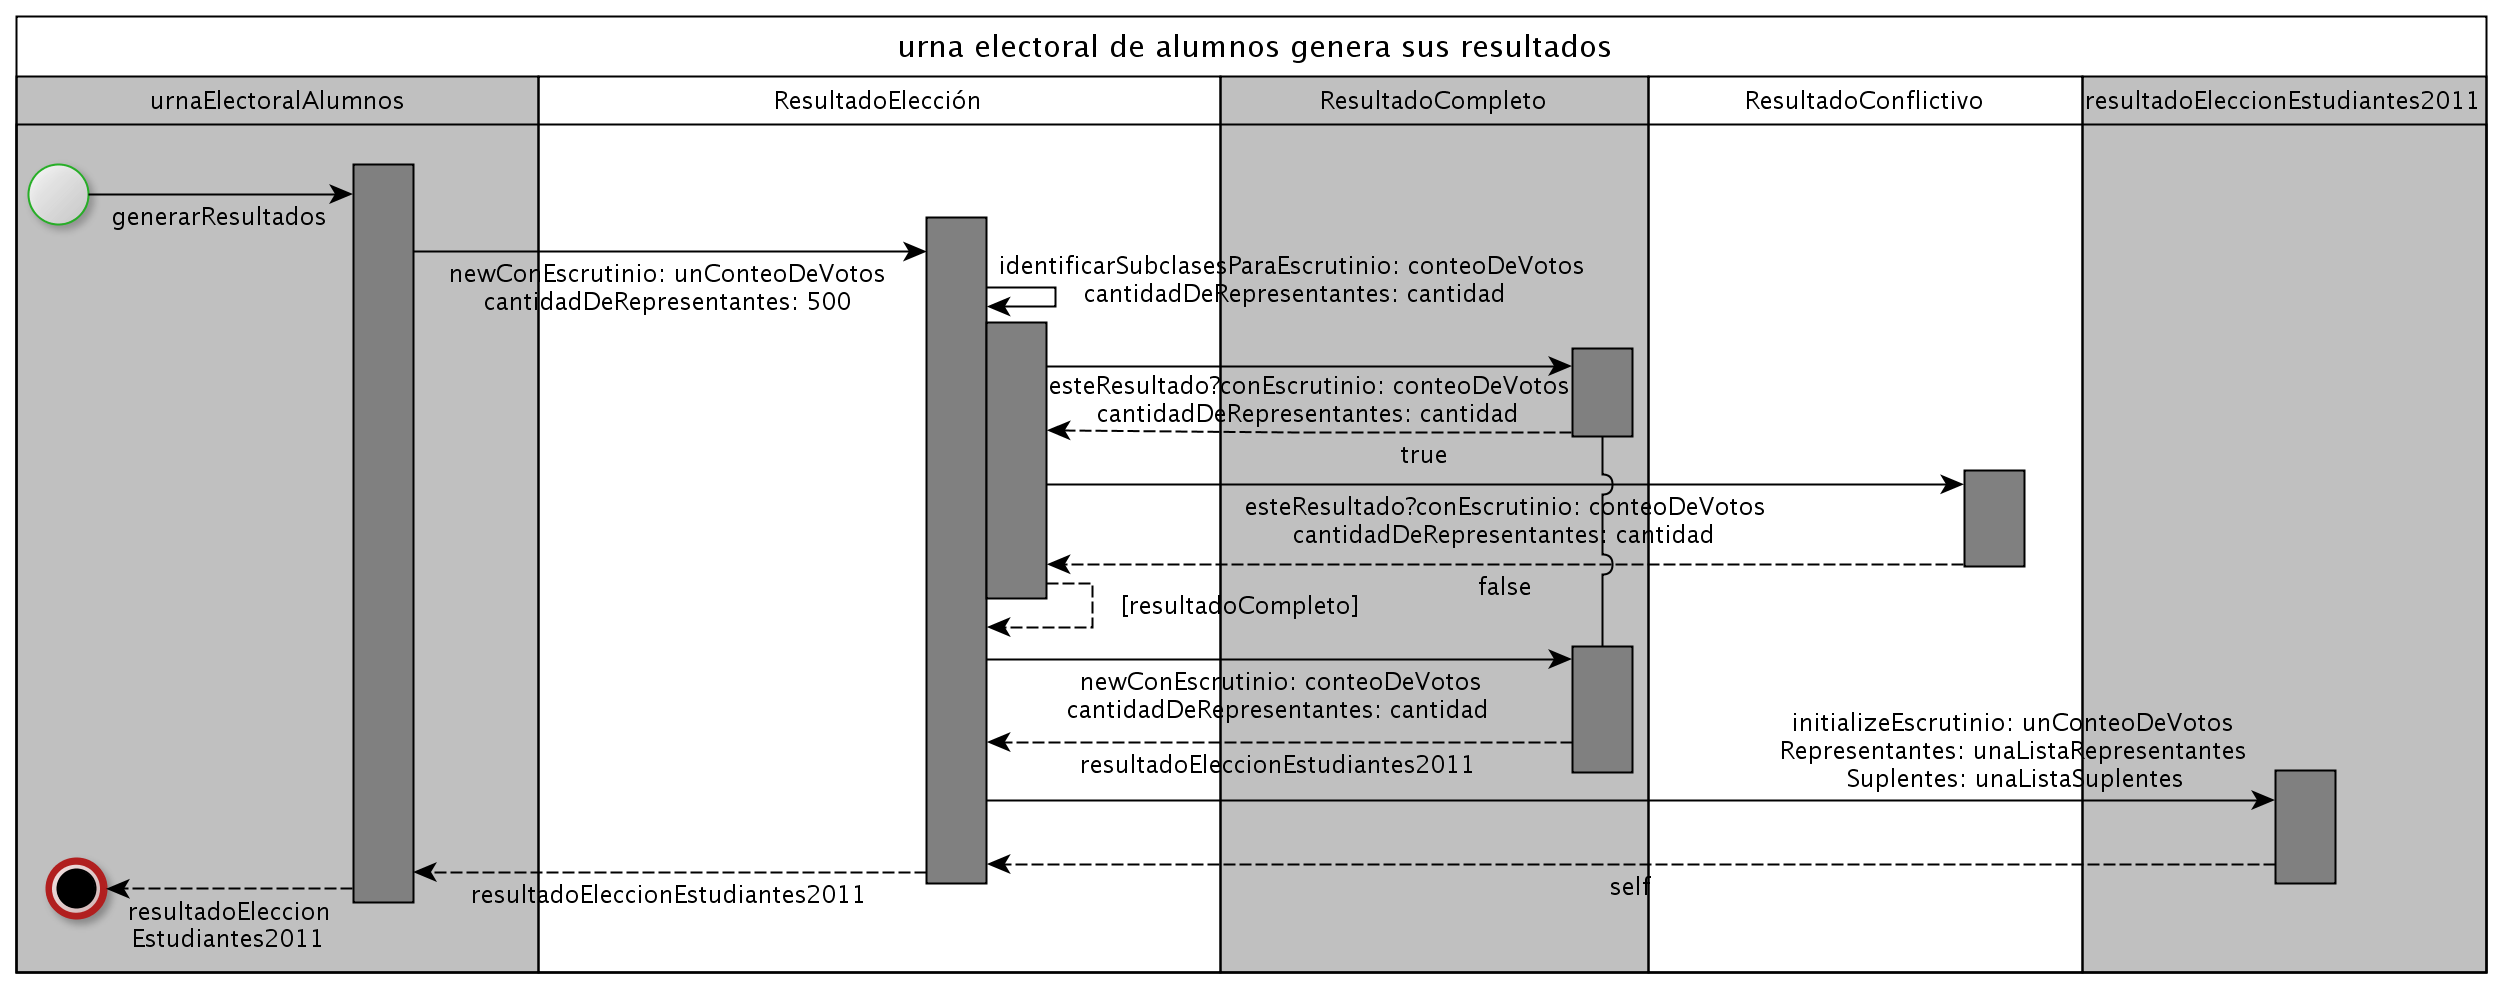
\includegraphics[scale=0.2]{diagramas/diagramaUrnaElectoralGeneraResultadosCompletos.png}
\end{center}


Por \'ultimo se presenta un diagrama de objetos que representan las relaciones de conocimiento entre los diferentes objetos.

\begin{center}
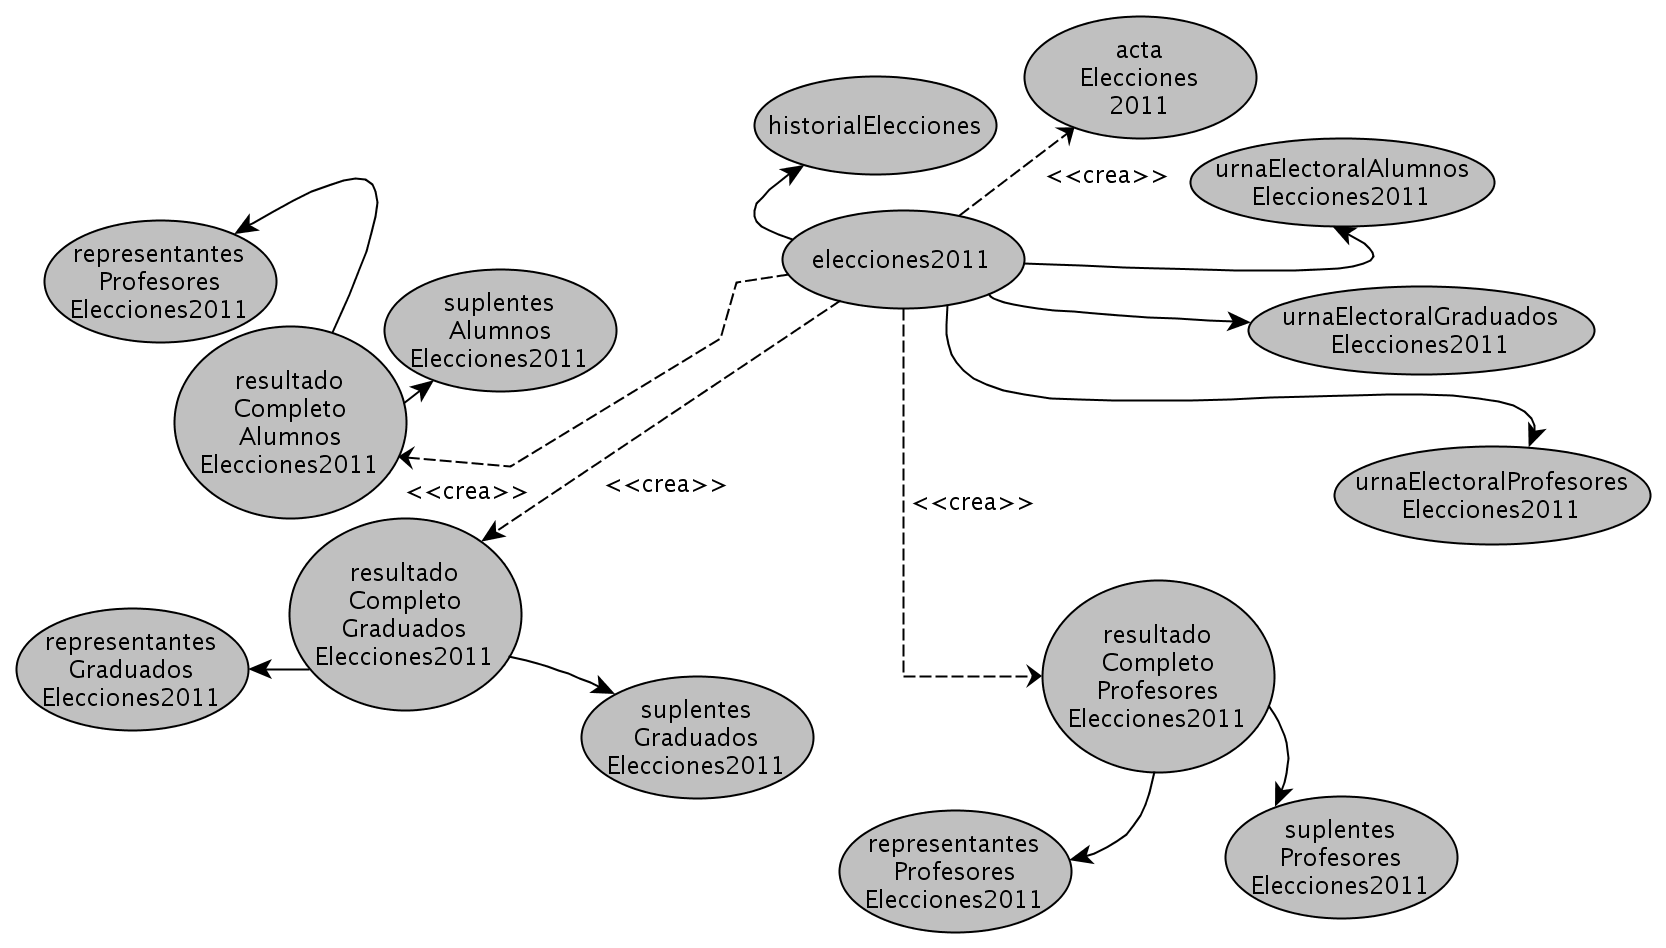
\includegraphics[scale=0.25]{diagramas/modeloDeObjetosResultados.png}
\end{center}